\documentclass[11pt,a4paper,roman]{scrartcl}
\usepackage{parskip}
\usepackage[english]{babel}
\usepackage{url}
\usepackage[utf8x]{inputenc}
\usepackage{amsmath}
\usepackage{amssymb}
\usepackage{graphicx}
\usepackage[export]{adjustbox}
\usepackage{listings}
\usepackage{float}
\usepackage{hyperref}
\usepackage[document]{ragged2e}
\usepackage{bm}
\usepackage[section]{placeins}
\title{Computer exercise 7}
\date{}
\author{Carl Ridnert, 940325-0712, ridnert@kth.se \\
Yue Jiao, 911024-7799, yj@kth.se}

\begin{document}

\maketitle
\begin{figure}[h]
\centering
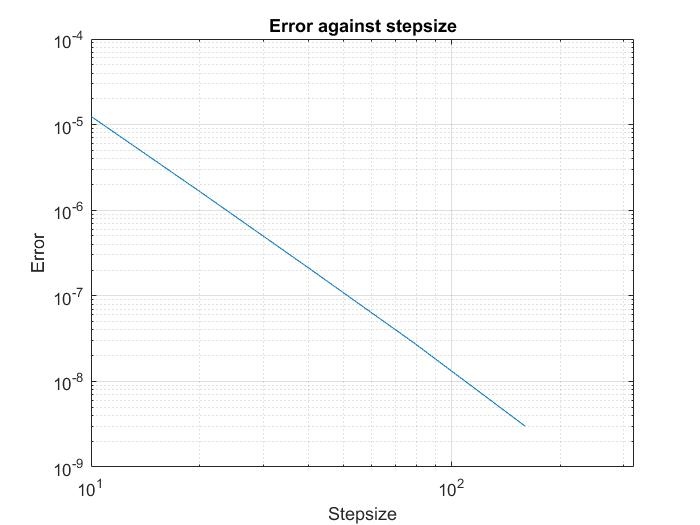
\includegraphics[width=0.45\textwidth,center]{1}
\end{figure}


\newpage

\section*{Part A}

\subsection*{a)}

In this computer exercise a matlab function is given which outputs $\boldsymbol{A}$ and $\boldsymbol{b}$ for some ill posed linear system of equations $\boldsymbol{Ax}=\boldsymbol{b}$.
In this problem we are estimating the condition number $\kappa (A)$ when the size of A is 8x8 using the following relation:

\begin{equation}
\frac{||\Delta \boldsymbol{x}||_2}{||\boldsymbol{x}||_2}=\kappa(A)\frac{||\Delta b||_2}{||\boldsymbol{b}||_2}
\end{equation}
This can be rewritten as

\begin{equation}
\kappa(A)=\frac{||\Delta \boldsymbol{x}||_2||\boldsymbol{b}||_2}{||\Delta b||_2 ||\boldsymbol{x}||_2}
\end{equation}

In order to obtain an estimate for $\kappa(A)$ we first compute the solution to the equation system $\boldsymbol{x}=\boldsymbol{A^{-1}}\boldsymbol{b}$. Then disturb $\boldsymbol{b}$ with some value $\Delta \boldsymbol{b}$ and solve the new equation system $\hat{\boldsymbol{x}}=\boldsymbol{A^{-1}}(\boldsymbol{b}+\Delta \boldsymbol{b})$, this gives $\Delta \boldsymbol{x}=\hat{\boldsymbol{x}}-\boldsymbol{x}$. Finally $\Delta \boldsymbol{x}, \boldsymbol{b},\boldsymbol{A}$ and $\Delta b$ are plugged into equation (2). This is repeated for 100 times for each randomly drawn $\Delta b$ of $order=O[10^{-12},10^{-13},10^{-14},10^{-15}]$ and the mean is taken for each order.

The results are the following: \\
The mean condition number when the $\Delta \boldsymbol{b}$ is around $10^{-12}$ is $2.603404\times 10^{12}$. \\
The mean condition number when the $\Delta \boldsymbol{b}$ is around $10^{-13}$ is $2.126989\times 10^{12}$. \\
The mean condition number when the $\Delta \boldsymbol{b}$ is around $10^{-14}$ is $2.139316\times 10^{12}$. \\
The mean condition number when the $\Delta \boldsymbol{b}$ is around $10^{-15}$ is $2.415286\times 10^{12}$. \\

The condition number calculated by the Matlab command $cond$ from matlabs built in function is $1.785061\times 10^{12}$. 
\subsection*{b)}

The condition number of a matrix $R$ is calculated experimentally by the following method. First a vector $\boldsymbol{x}$ is generated randomly with elements between 0 and 1 and the length equal to the number of column of $R$. Let vector $\boldsymbol{b}$ be $\boldsymbol{b} = R\cdot\boldsymbol{x}$. Then vectors $\Delta \boldsymbol{b}$ are generated randomly with the size of $\boldsymbol{b}$ and elements between $0$ and $10^{-15}$. Then the following equations are solved for each of these vectors $\Delta \boldsymbol{b}$: $A\cdot \boldsymbol{x}_{new} =\boldsymbol{b} + \Delta \boldsymbol{b}$ with Gaussian elimination. The change in $\boldsymbol{x}$ shall be $\Delta \boldsymbol{x} = \boldsymbol{x}_{new} - \boldsymbol{x}$ and the experimental condition number can be calculated with the equation discussed above. The residual of a matrix $A$ is calculated by the method describe in part a) as $\boldsymbol{res} = A \hat{\boldsymbol{x}} - \boldsymbol{b}$. 

The experimental results are compare with the results calculated with Matlab functions $cond$. 

The results: \\
When rank is 8 \\
\quad	 norm(E): 0 \\
\quad	 cond(R11): $ 1.587780 \times  10^{12}$ \\
\quad	 Experimental condition number of R11: $4.158030 \times  10^{11}$ \\
\quad	 norm(x): 1.455359 \\
\quad	 norm(res):  $8.308148 \times  10^{-16}$ \\
When rank is 7 \\
\quad	 norm(E): $ 5.074438 \times  10^{12}$ \\
\quad	 cond(R11): $4.709339 \times  10^{9}$ \\
\quad	 Experimental condition number of R11: $1.339585 \times  10^{9}$ \\
\quad	 norm(x): 1.455359 \\
\quad	 norm(res): $2.752749 \times  10^{-12}$ \\
When rank is 6 \\
\quad	 norm(E): $1.707062 \times  10^{-9}$ \\
\quad	 cond(R11): $1.804057 \times  10$ \\
\quad	 Experimental condition number of R11: 5.850346 \\
\quad	 norm(x): 1.455359 \\
\quad	 norm(res): $5.372663 \times  10^{-11}$ \\
When rank is 5 \\
\quad	 norm(E): $3.602908 \times  10^{-1}$ \\
\quad	 cond(R11): 6.192847 \\
\quad	 Experimental condition number of R11: 3.568354 \\
\quad	 norm(x): 1.455359 \\
\quad	 norm(res): $ 1.728147 \times  10^{-1}$ \\

We note that when the rank is decreased, the condition of the matrix gets lower, indicating that the system is more robust to disturbances. However, this also implies that the norm of the residual grows which indicates that the solution is less precise. There seems to be a tradeoff in the condition of a system and the norm of the residual. 

\section*{Part B}
In this part, data fitting is performed using least squares method. A file containing data of 288 months of $CO_2$ measurements in the atmosphere is provided. The parameters $c_1$, $c_2$, $a_k$ and $b_k$ shall be decided so the following function shall fit the data with the minimum 2-norm of the residual. 
\begin{equation}
y(t) = c_1 + c_2 e^{\alpha t} + \sum_{k=1}^{n}(a_k cos(\frac{2\pi k t}{12}) + b_k sin(\frac{2\pi k t}{12})), \quad \alpha = 0.00037
\end{equation}
The function is a linear expression of variables $c_1, c_2, a_k, b_k$. This means we can write (3) as a linear system of equations as $Ax = b$. The A matrix can be formulated as follows:
\begin{equation*}
A = \begin{bmatrix}
1, e^{\alpha t_1}, \cos\left(\frac{2\pi t_1\times 1}{12}\right), \sin\left(\frac{2\pi t_1\times 1}{12}\right), \cos\left(\frac{2\pi t_1\times 2}{12}\right), \sin\left(\frac{2\pi t_1\times 2}{12}\right), ... , \cos\left(\frac{2\pi t_1\times n}{12}\right), \sin\left(\frac{2\pi t_1\times n}{12}\right) \\
1, e^{\alpha t_2}, \cos\left(\frac{2\pi t_2\times 1}{12}\right), \sin\left(\frac{2\pi t_2\times 1}{12}\right), \cos\left(\frac{2\pi t_2\times 2}{12}\right), \sin\left(\frac{2\pi t_2\times 2}{12}\right), ... , \cos\left(\frac{2\pi t_2\times n}{12}\right), \sin\left(\frac{2\pi t_2\times n}{12}\right) \\
\vdots \\
1, e^{\alpha t_m}, \cos\left(\frac{2\pi t_m\times 1}{12}\right), \sin\left(\frac{2\pi t_m\times 1}{12}\right), \cos\left(\frac{2\pi t_m\times 2}{12}\right), \sin\left(\frac{2\pi t_m\times 2}{12}\right), ... , \cos\left(\frac{2\pi t_m\times n}{12}\right), \sin\left(\frac{2\pi t_m\times n}{12}\right) \\
\end{bmatrix}
\end{equation*}
with the coefficients ordered as:
\begin{equation*}
x = \begin{bmatrix} c_1, c_2, a_1, b_1, a_2, b_2, ..., a_n, b_n \end{bmatrix}^T
\end{equation*}
and the functional values
\begin{equation*}
b = \begin{bmatrix} y(t_1), y(t_2), ... ,y(t_m) \end{bmatrix}^T.
\end{equation*}

Three different cases are calculated, i.e. $n = 1,2,3$. The method used is data-fitting with QR-factorization. This means that the following procedure is performed: 

Perform QR-factorization on A to calculate Q, R, P such that: $AP = QR$. Then calculate the vector $\hat{d} = Q^T b$. Then use Gaussian elimination to solve the equation $R \hat{y} = \hat{d}$ to get $\hat{y}$. At last, the parameters $\hat{x}$ which fit the data in such a way that minimize the 2-norm of the residual can be calculated by $\hat{x} = P\hat{y}$. The norm of the residual is then $res = A\hat{x} - b$. Then we shall get the following results: 

The 2-norm residual when $k=1$ is: 15.203572

The 2-norm residual when $k=2$ is: 11.393595

The 2-norm residual when $k=3$ is: 11.297228

So the smallest residual is archived when $k=3$. The following plot shows the fitting to the data. 

\begin{figure}[H]
\centering
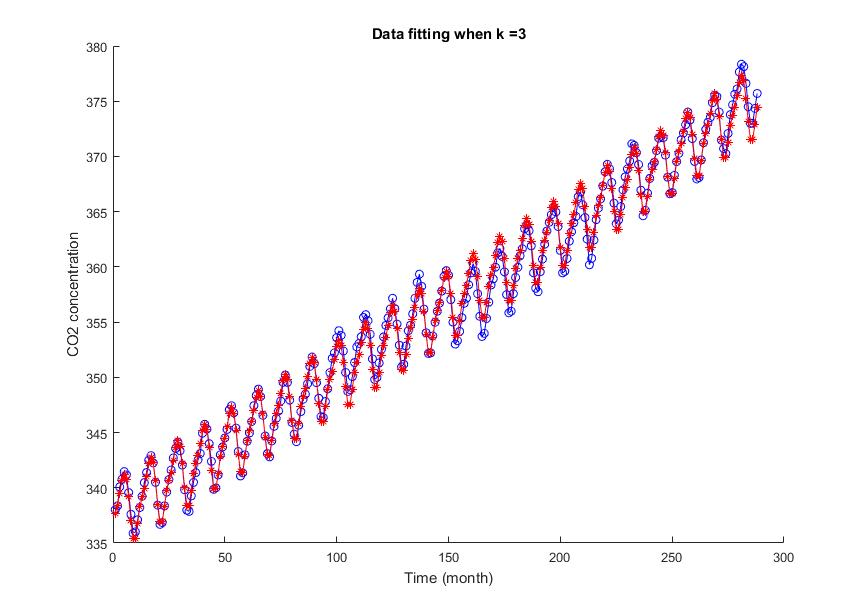
\includegraphics[width=0.9\textwidth,center]{b3}
\caption{Plots of data fitting when $k=3$}. 
\end{figure}

\end{document}

%% First part
%% a
clear, clc;
n = 8;
[A, b] = illposed(n);
x = A\b;
c = 100;
for s = [10^-12 10^-13 10^-14 10^-15]
  k = zeros(1, c);
  for i = 1:c
    deltab = rand(n,1)*s;
    xnew = A\(b+deltab);
    k(i) = (norm(xnew-x)/norm(x))/(norm(deltab)/norm(b));
  end
  fprintf('The mean condition number when the deltab is around %e is %e.\n', s, mean(k))
end

%% b
[A, b] = illposed(8);
format long
for r = [8 7 6 5]
  [Q, R, P] = qr(A);
  R11 = R(1:r, 1:r);
  E = R(r+1:8, r+1:8);
  fprintf('When rank is %d\n', r);
  fprintf('\t norm(E): %e\n', norm(E))
  fprintf('\t cond(R11): %e\n', cond(R11))
  np = 20;
  cp = 100;
  ck = zeros(np, 1);
  for i = 1:np
    xp = rand(r,1);
    bp = R11*xp;
    kp = zeros(1, cp);
    for j = 1:cp
      deltabp = rand(r,1).*10^-15;
      xnewp = R11\(bp+deltabp);
      kp(j) = (norm(xnewp-xp)/norm(xp))/(norm(deltabp)/norm(bp));
    end
    ck(i) = mean(kp);
  end
  fprintf('\t Experimental condition number of R11: %e\n', mean(ck))
  fprintf('\t norm(x): %e\n', norm(A\b))
  D = Q'*b;
  dt = D(1:r);
  yt = R11\dt;
  xt = P*([yt; zeros(8-r, 1)]);
  res = A*xt - b;
  fprintf('\t norm(res): %e\n', norm(res))
end

%% Second part
load('manualoa8000.dat')
%pick out the monthly values (column 2:13) and store columnwise in Q
Q=manualoa8000(:,2:13)';
b=Q(:); %all measurements are in time increasing order in one column
m=length(b);
t=[1:m]';
%plot(t,b,'x');
tend = m;
range = ones(m,1);
alpha = 0.00037;
for k = 1:3
    A = [range, exp(alpha*t)];
    for i = 1:k
        A = [A, cos(2*pi*i*t/12), sin(2*pi*i*t/12)];
    end
    [Q, R, P] = qr(A);
    d = Q'*b;
    y = R\d;
    x = P*y;
    bfit = A*x;
    res = abs(bfit-b);
    x = A\b;
%     bfit2 = x(1)*range + x(2)*exp(alpha*t);
%     for i = 1:k
%         bfit2 = bfit2 + x(3+(i-1)*2)*cos(2*pi*i*t/12) + x(4+(i-1)*2)* sin(2*pi*i*t/12);
%     end
    figure();
    hold on;
    plot(t, b, 'bo-');
    plot(t, bfit, 'r*-');
    title(strcat('Data fitting when k = ', num2str(k)));
    xlabel('Time (month)');
    ylabel('CO2 concentration');
    %plot(t, bfit2, 'g.-');
    fprintf('The 2-norm residual when k=%d is: %f\n', k, norm(res));
end